\chapter{Numeryczne metody estymacji}\label{numPAJ}

Odkąd zjawiska przyrodnicze zaczęto opisywać przy użyciu formalizmu matematycznego,
pojawiła się potrzeba rozwiązywania zadań analizy matematycznej czy algebry. Dopóki były
one nieskomplikowane, dawały się rozwiązywać analitycznie, tzn. z użyciem pewnych
przekształceń algebraicznych prowadzących do otrzymywania rozwiązań. Z czasem jednak, przy powstawaniu coraz to bardziej skomplikowanych teorii
opisujących zjawiska, problemy te stawały się na tyle złożone, iż ich rozwiązywanie ścisłe
było albo bardzo czasochłonne albo też zgoła niemożliwe. Przez numerykę rozumie się dziedzinę matematyki
zajmującą się przybliżonym rozwiązywaniem zagadnień algebraicznych. Pozwalała ona znajdować ich 
przybliżone rozwiązania z żądaną dokładnością. Podstawową zaletą wykorzystywania przybliżonych rozwiązań była ogólność
formułowanych algorytmów, tzn. w ramach danego zagadnienia nie miało znaczenia czy było
ono proste czy też bardzo skomplikowane (najwyżej wiązało się z większym nakładem pracy
obliczeniowej), natomiast wadą była czasochłonność. Dlatego prawdziwy renesans metod
numerycznych nastąpił wraz z powszechnym użyciem w pracy naukowej maszyn cyfrowych oraz komputerów \citep{milewski}. 

Dziś dziesiątki żmudnych dla człowieka operacji
arytmetycznych wykonuje komputer, jednak złożoność obliczeniowa algorytmów uczenia maszynowego stała się krytycznym czynnikiem ograniczającym prace w sytuacjach, gdy rozważane są duże zbiory danych. Te ograniczenia spowodowały, że w modelowaniu statystycznym wielkiej skali zaczęto wykorzystywać algorytmy \textbf{stochastycznego spadku gradientu}. 

W poniższym rozdziale przedstawione są klasyczne algorytmy spadku wzdłuż gradientu Cauchy'ego oraz Raphsona-Newtona. Następnie omówiony jest algorytm stochastycznego spadku wzdłuż gradientu, którego zastosowanie do estymacji współczynników w modelu Coxa jest kluczowym celem pracy. Algorytm stochastycznego spadku gradientu to metoda optymalizacji używana w sytuacjach, gdy rozważaną funkcję można zapisać jako sumę różniczkowalnych składników. Ponieważ popularne metody statystycznej estymacji, takie jak \textit{Fisher scoring}, algorytm \textit{Expectation–maximization} czy iteracyjna ważona metoda najmniejszych kwadratów \citep{fisher3,dempster,greenPJ} nie zawsze przenoszą się na zastosowania do danych dużej skali bądź danych napływających (\textit{ang. streaming data}), niekiedy algorytm stochastycznego spadku gradientu jest jedyną dostępną metodą optymalizacji numerycznej. Ponadto przedstawiono również zalety algorytmów stochastycznego spadku gradientu, które przemawiają za atrakcyjnością i popularnością tego typu rozwiązania. Omawiane pojęcia oparto o \cite{bott1,bott2}, \cite{kotlowski} oraz \cite{fortuna}.

\newpage
\section{Algorytmy spadku wzdłuż gradientu}\label{R-N}

Poniższy rozdział przedstawia popularne iteracyjne algorytmy wyznaczania przybliżonej wartości miejsca zerowego funkcji oraz rozważaną w pracy metodę stochastycznego spadku gradientu. Szukanie miejsc zerowych funkcji jest przydatne w problemach optymalizacyjnych, gdy celem jest znalezienie pierwiastka pochodnych badanej funkcji. Dodatkowo takie algorytmy wykorzystywane są do rozwiązywania (nieliniowych) układów równań. Metody iteracyjne składają się zazwyczaj z $k$ kroków bądź są zatrzymywane, gdy osiągnięty zostanie warunek stopu, czyli gdy odległość pomiędzy kolejnymi przybliżeniami jest dość mała $\parallel w_{k+1}-w_k\parallel < \varepsilon$ lub wartość gradientu funkcji w wyznaczonym punkcie jest bliska wektorowymi zerowemu $\parallel \nabla_Q(\mathbf{w_k}) \parallel \leqslant \varepsilon$ (test stacjonarności), gdzie $\varepsilon$ to zadana z góry precyzja.
Metoda stochastycznego spadku wzdłuż gradientu zakłada, że minimalizowaną funkcję $Q(w)$ można przedstawić jako różniczkowalną sumę jej składników $Q(w) = \sum_{i=1}^{n}Q_i(w)$. W~poniższych algorytmach $\alpha_k$ oznacza długość kroku algorytmu.
\begin{center}
\textbf{Metoda spadku wzdłuż gradientu I (Cauchy’ego)}
\end{center}
Minimalizacja funkcji $Q(w)$:
\begin{itemize}
\item Zaczynamy od wybranego rozwiązania startowego, np. $w_{0} = 0$.
\item Dla $k = 1, 2, \dots$ aż do zbieżności
	\begin{itemize}
	\item Wyznaczamy gradient w punkcie $w_{k-1}, \nabla_{Q}(w_{k-1})$.
	\item Robimy krok wzdłuż negatywnego gradientu: $$w_{k} = w_{k-1} - \alpha_{k}\nabla_{Q}(w_{k-1}). $$
	\end{itemize}
\end{itemize}

\begin{center}
\textbf{Metoda spadku wzdłuż gradientu II (Newtona-Raphsona)}
\end{center}
Minimalizacja funkcji $Q(w)$:
\begin{itemize}
\item Zaczynamy od wybranego rozwiązania startowego, np. $w_{0} = 0$.
\item Dla $k = 1, 2, \dots$ aż do zbieżności
	\begin{itemize}
	\item Wyznaczamy~gradient~w~punkcie~$w_{k-1}, \nabla_{Q}(w_{k-1})$~i~odwrotność~$(D_{Q}^{2}(w_{k-1}))^{-1}$.
	\item Robimy krok wzdłuż negatywnego gradientu z zadanym krokiem przez Hesjan: 
	\begin{equation}\label{NJU-rap}
	 w_{k} = w_{k-1} - (D_{Q}^{2}(w_{k-1}))^{-1}\nabla_{Q}(w_{k-1}). 
	 \end{equation}	
	\end{itemize}
\end{itemize}
\begin{center}
\textbf{Metoda stochastycznego spadku wzdłuż gradientu I}
\end{center}
Minimalizacja funkcji $Q(w)$:
\begin{itemize}
\item Zaczynamy od wybranego rozwiązania startowego, np. $w_{0} = 0$.
\item Dla $k = 1, 2, \dots$ aż do zbieżności
	\begin{itemize}
	\item Wylosuj $i \in \{1,\dots,n\}$
	\item Wyznaczamy gradient funkcji $Q_{i}$ w punkcie $w_{k-1}, \nabla_{Q_{i}}(w_{k-1})$.
	\item Robimy krok wzdłuż negatywnego gradientu: 
	\begin{equation}\label{sgdrownanie}
	 w_{k} = w_{k-1} - \alpha_{k}\nabla_{Q_{i}}(w_{k-1}).
	  \end{equation}
	\end{itemize}
\end{itemize}

\section{Algorytm stochastycznego spadku wzdłuż gradientu I}\label{SGD}
\vspace{-5pt}
Stochastyczny spadek gradientu jest często stosowany do estymacji współczynników w szerokiej gamie modeli uczenia maszynowego, takich jak maszyny wektorów podpierających (\textit{ang. Support Vector Machines}), regresja logistyczna czy modele graficzne~\citep{finkel}. W~połączeniu z algorytmem propagacji wstecznej jest standardową metodą w procesie tworzenia sztucznych sieci neuronowych. Algorytm stochastycznego spadku gradientu był używany już od 1960 przy estymacji współczynników w modelu regresji liniowej \citep{ADALINE} oraz był  wykorzystywany w algorytmie filtrów adaptacyjnych najmniejszych średnich kwadratów \citep{widrow2} (\textit{ang.~least mean squares (LMS) adaptive filter}).

Idea algorytmu stochastycznego spadku gradientu jest następująca: zamiast obliczać gradient na całej funkcji $Q(w)$, w danym kroku oblicz
gradient tylko na pojedynczym elemencie $Q_{i}(w)$. Nazwa \textit{stochastyczny} bierze się stąd, iż oryginalnie wybiera
się $Q_{i}(w)$ losowo. W praktyce zwykle przechodzi się po całym zbiorze danych w losowej kolejności.
%\vspace{-10pt}
\subsubsection{Właściwości stochastycznego spadku wzdłuż gradientu}
%\vspace{-5pt}
Zbieżność algorytmu stochastycznego spadku gradientu była szeroko badana w literaturze aproksymacji stochastycznych. Aby uzyskać zbieżność zazwyczaj wymaga się, aby ciąg kroków $\alpha_k$ był malejący i spełniał warunki $\sum\nolimits_k \alpha_k = \infty$ oraz $\sum\nolimits_k \alpha_k^2 < \infty$~(\cite{bott1}).
Twierdzenie Robbinsa-Siegmunda \citep{robbins} przy łagodnych warunkach zapewnia~zbieżność~prawie na pewno \citep{bottDOD}, nawet  gdy~optymalizowana~funkcja~nie~jest~wszędzie~różniczkowalna.

Prędkość zbieżności stochastycznego spadku gradientu jest w rzeczywistości ograniczana przez zgrubną (\textit{ang. noisy}) aproksymacje prawdziwego gradientu. Gdy długości kroków algorytmu
maleją zbyt wolno, wariancja estymatorów parametrów $w_k$ maleje równie wolno. Gdy kroki maleją
zbyt szybko, wartości oczekiwane estymatorów $w_k$ potrzebują więcej czasu by osiągnąć optimum \citep{bott1}. Pod pewnymi warunkami regularności \citep{murata}, najlepsza prędkość zbieżności jest uzyskana dla ciągu kroków $\alpha_k\sim k^{-1}$.

Jak wykazano w \cite{dennis} pod pewnymi odpowiednimi warunkami regularności, gdy zainicjowany współczynnik początkowy $w_0$ jest wystarczająco blisko optimum i krok algorytmu jest odpowiednio mały, algorytm stochastycznego spadku gradientu osiąga liniową zbieżność. Oznacza to, iż przy spełnieniu założeń metody, odległości pomiędzy kolejnymi przybliżeniami a minimum funkcji $\mathbf{w^{\ast}}$ maleją liniowo: $\parallel \mathbf{w^{\ast}} - \mathbf{w_{k+1}} \parallel \leqslant c \parallel \mathbf{w^{\ast}} - \mathbf{w_k} \parallel$. Zbieżność wymaga często przejścia parokrotnie po całym
zbiorze danych. Wady i zalety algorytmu wymienione są poniżej. Zalety~zdecydowanie przewyższają~wady.

\textbf{Zalety} \vspace{-5pt}
\begin{itemize}
\item \textcolor{orange}{Szybkość kroku}: obliczenie gradientu wymaga wzięcia tylko jednej
obserwacji.
\item \textcolor{orange}{Skalowalność}: cały zbiór danych nie musi nawet znajdować się
w pamięci operacyjnej.
\item \textcolor{orange}{Prostota}: gradient funkcji  $Q_{i}$ daje bardzo prosty wzór na
modyfikacje wag.
\end{itemize}

\textbf{Wady}  \vspace{-5pt}
\begin{itemize}
\item \textcolor{orange}{Wolna zbieżność}: czasem gradient stochastyczny do zbieżności wymaga wielu iteracji po zbiorze uczącym.
\item \textcolor{orange}{Problem z ustaleniem długości kroku $k$}: wyznaczenie $k$
przez przeszukiwanie liniowe nie przynosi dobrych rezultatów,
ponieważ nie optymalizujemy oryginalnej funkcji $Q$ tylko jej jeden
składnik $Q_{i}$.
\end{itemize}
\newpage
\section{Porównanie algorytmów spadku wzdłuż gradientu}

W niniejszym podrozdziale przedstawiono graficznie różnice w wyborze kolejnych punktów w trakcie optymalizacji między omawianymi w poprzedniej części pracy algorytmami spadku wzdłuż gradientu I (Cauchy'ego), spadku wzdłuż gradientu II (Newtona-Raphsona) oraz stochastycznego spadku wzdłuż gradientu I. W celu zobrazowania przykładu na dwuwymiarowym wykresie, postanowiono ograniczyć się do modelu z jedną zmienną objaśniającą i wyrazem wolnym. Do przykładu wybrano model regresji logistycznej, z racji na prostotę przedstawienia funkcji log-wiarogodności jako sumy różniczkowalnych składników.

Funkcja log-wiarogodności dla regresji logistycznej \citep{czepiel, dobson} to
\begin{equation}\label{logglm}
\ell(\beta_1,\beta_2) = \sum\limits_{i=1}^{N} Q_i(\beta_1,\beta_2), 
\end{equation}
\begin{equation}
Q_i(\beta_1,\beta_2) = y_i(\beta_1+\beta_2x_i) -\log(1+\exp(\beta_1+\beta_2x_i)).
\end{equation}

Wtedy współrzędne gradientu funkcji wiarogodności to odpowiednio

\begin{equation*}
\dfrac{\partial\ell(\beta)}{\partial\beta_1} = \sum\limits_{i=1}^{N}\Big(y_i-\pi_i(\beta)\Big), \ \ \
\dfrac{\partial\ell(\beta)}{\partial\beta_2} = \sum\limits_{i=1}^{N}x_i\Big(y_i-\pi_i(\beta)\Big), \ \ \
\pi_i(\beta) = \frac{\exp(\beta_1+\beta_2x_i)}{1+\exp(\beta_1+\beta_2x_i)},
\end{equation*}

zaś macierz informacji wyraża się jak następuje
\begin{equation}\label{iii}
\mathscr{I}(\beta) = 
\begin{bmatrix}
    \sum\limits_{i=1}^{N}\pi_i(\beta)(1-\pi_i(\beta))       & \sum\limits_{i=1}^{N}x_i\pi_i(\beta)(1-\pi_i(\beta)) \\
\sum\limits_{i=1}^{N}x_i\pi_i(\beta)(1-\pi_i(\beta)) & \sum\limits_{i=1}^{N}x_i^2\pi_i(\beta)(1-\pi_i(\beta)) 
\end{bmatrix},
\end{equation}
gdzie $N$ to liczba obserwacji.

Aktualizacja kandydata na miejsce zerowe w $k$-tym kroku algorytmu optymalizacyjnego wśród kolejnych metod omówionych w rozdziale (\ref{R-N}) wyraża się poniższymi wzorami
\\
\begin{center}
\textbf{Metoda spadku wzdłuż gradientu I (Cauchy’ego)}
\end{center}
\begin{equation*}
\beta_{k} = \beta_{k-1} + \alpha_{k}\cdot\Big(\sum\limits_{i=1}^{N}(y_i-\pi_i(\beta_{k-1})), \sum\limits_{i=1}^{N}x_i(y_i-\pi_i(\beta_{k-1}))\Big).
\end{equation*}
\begin{center}
\textbf{Metoda spadku wzdłuż gradientu II (Newtona-Raphsona)}
\end{center}
\begin{equation*}
\beta_{k} = \beta_{k-1} + \mathscr{I}(\beta_{k-1})^{-1}\cdot\Big(\sum\limits_{i=1}^{N}(y_i-\pi_i(\beta_{k-1})), \sum\limits_{i=1}^{N}x_i(y_i-\pi_i(\beta_{k-1}))\Big),
\end{equation*}
gdzie $\mathscr{I}(\beta_{k-1})$ zdefiniowane jest we wzorze (\ref{iii}). 
\begin{center}
\textbf{Metoda stochastycznego spadku wzdłuż gradientu I}
\end{center}
\begin{equation*}
\beta_{k} = \beta_{k-1} + \alpha_{k}\cdot\Big(y_i-\pi_i(\beta_{k-1}), x_i(y_i-\pi_i(\beta_{k-1}))\Big),
\end{equation*}
gdzie $i$ to indeks wylosowanej obserwacji w danym kroku.
\\ \ \\
Ponieważ algorytmy te znajdują minimum funkcji, a docelowo szukane jest maksimum, stąd wykorzystano przeciwieństwo funkcji log-wiarogodności. Dlatego w wyżej wymienionych wzorach zmieniono znaki przed pochodnymi na przeciwne.

\newpage
\subsubsection{Symulacje trajektorii zbieżności algorytmów}
Poniższymi wywołaniami kodów z pakietu $\mathcal{R}$ można wygenerować 10000 obserwacji z rozkładu jednostajnego i na ich podstawie wygenerować 10000 obserwacji z rozkładu dwupunktowego o takim rozkładzie prawdopodobieństwa sukcesu, by rzeczywiste współczynniki w modelu regresji logistycznej dla tych zmiennych wynosiły odpowiednio: 2 dla wyrazu wolnego oraz 3 dla zmiennej objaśniającej z rozkładu jednostajnego. 
\begin{Shaded}
\begin{Highlighting}[]
\NormalTok{x <-}\StringTok{ }\KeywordTok{runif}\NormalTok{(}\DecValTok{10000}\NormalTok{)}
\NormalTok{z <-}\StringTok{ }\DecValTok{2} \NormalTok{+}\StringTok{ }\DecValTok{3}\NormalTok{*x}
\NormalTok{pr <-}\StringTok{ }\DecValTok{1}\NormalTok{/(}\DecValTok{1}\NormalTok{+}\KeywordTok{exp}\NormalTok{(-z))}
\NormalTok{y <-}\StringTok{ }\KeywordTok{rbinom}\NormalTok{(}\DecValTok{10000}\NormalTok{,}\DecValTok{1}\NormalTok{,pr)}
\end{Highlighting}
\end{Shaded}

Tak zasymulowane dane wprowadzono do przygotowanej funkcji \texttt{logitGD()}, dzięki której można śledzić wartości ekstremum w kolejnych krokach omawianych algorytmów. Kody funkcji \texttt{logitGD()} oraz \texttt{graphSGD()} tworzącej wykresy porównujące trajektorie zbieżności różnych algorytmów spadku gradientu  dostępne są w Dodatku~\ref{kody}. Wyniki wywołań funkcji \texttt{graphSGD()} zostały umieszczone na Rysunkach \ref{fig:sc5asd} - \ref{fig:sc4asd}.

Na każdym z wykresów na osi $OX$ pokazano wartości współczynnika dla zmiennej objaśniającej w kolejnych krokach poszczególnych algorytmów. Na osi $OY$ zaznaczono współczynnik wyrazu wolnego. Punkt startowy oznaczono na wykresie czarnym trójkątem, a~czarnym kwadratem zaznaczono ekstremum funkcji log-wiarogodności, wyliczone dzięki funkcji \texttt{glm()} \citep{glmglm}, która do estymacji używa algorytmu iteracyjnej ważonej metody najmniejszych kwadratów. Ta metoda w regresji logistycznej jest równoważna algorytmowi \textit{Fisher's Scoring} \citep{scoring1, scoring2}, który używa obserwowanej macierzy Informacji Fishera (Definicja \ref{inf:fish}) w miejscu Hesjanu w algorytmie Newtona-Raphsona~(\ref{NJU-rap})). Trajektorie zbieżności do minimum w odrębnych algorytmach zaznaczono oddzielnymi kolorami. Dodatkowo wpisano liczbę kroków wymaganą przez algorytm do zbieżności. Przez \texttt{GDI} oznaczono algorytmu spadku gradientu rzędu I, zaś przez \texttt{GDII} rzędu II. Oznaczenie \texttt{SGD.i} odpowiada 3 algorytmom stochastycznego spadku gradientu o~różnych ciągach odpowiedzialnych za długość kroku. Indeks $i$ odpowiada ciągowi wybranemu do wyznaczania długości kroku algorytmu na zasadzie $\alpha_{k,i} = i/\sqrt{k}$.

\textbf{Warunki zbieżności}

W trakcie każdej symulacji postawiono pewne warunki konieczne do zbieżności. Ustalono maksymalną liczbę iteracji na 10001, gdzie przez pierwszy krok rozumiano start z punktu startowego. Dodatkowo warunek stopu ustalono na $\varepsilon=10^{-5}$ oraz ustalono ciąg odpowiadający długościom kroków w algorytmie spadku gradientu rzędu I \texttt{GDI} na $\alpha_{k} = 1/1000\sqrt{k}$. Symulacje powtórzono czterokrotnie, biorąc różne punkty startu algorytmów $$\beta_0 = (0,0), (1,2), (3.5,1), (4,3.2).$$

Ponieważ każda trajektoria w procesie estymacji metodą stochastycznego gradientu przy tych samych parametrów zbieżności jest inna, z racji na losową kolejność obserwacji, toteż dla każdego z czterech ustalonych punktów startowych zdecydowano się zobrazować symulację dwukrotnie, aby móc przedstawić stochastyczny aspekt tej metody. Symulacja nr 1 bazowała na losowym wzięciu punktów do algorytmów stochastycznego spadku gradientu, gdy ziarno losowania było ustawione na 4561, zaś w symulacji nr 2 ziarno ustawiono na 456.

\newpage

Ponieważ na Rysunkach \ref{fig:scasd} - \ref{fig:sc4asd} każda z symulacji ma inny zakres osi na wykresie, postanowiono na Rysunku \ref{fig:sc5asd} przygotować zestawienie podobnych symulacji przedstawiając trajektorie zbieżności na wspólnym zakresie osi. Miało to na celu uwypuklić skalę różnic w~długościach kroków algorytmów w zależności od odległości punktu startowego od rzeczywistego ekstremum. Dodatkowo na osiach zaznaczono warstwice funkcji log-wiarogodności w~modelu regresji logistycznej (równanie (\ref{logglm})).

\begin{figure}[h!]
  %\vspace{-10pt}
  \begin{center}
   \begin{subfigure}[h!]{0.49\textwidth}
%     \centering
     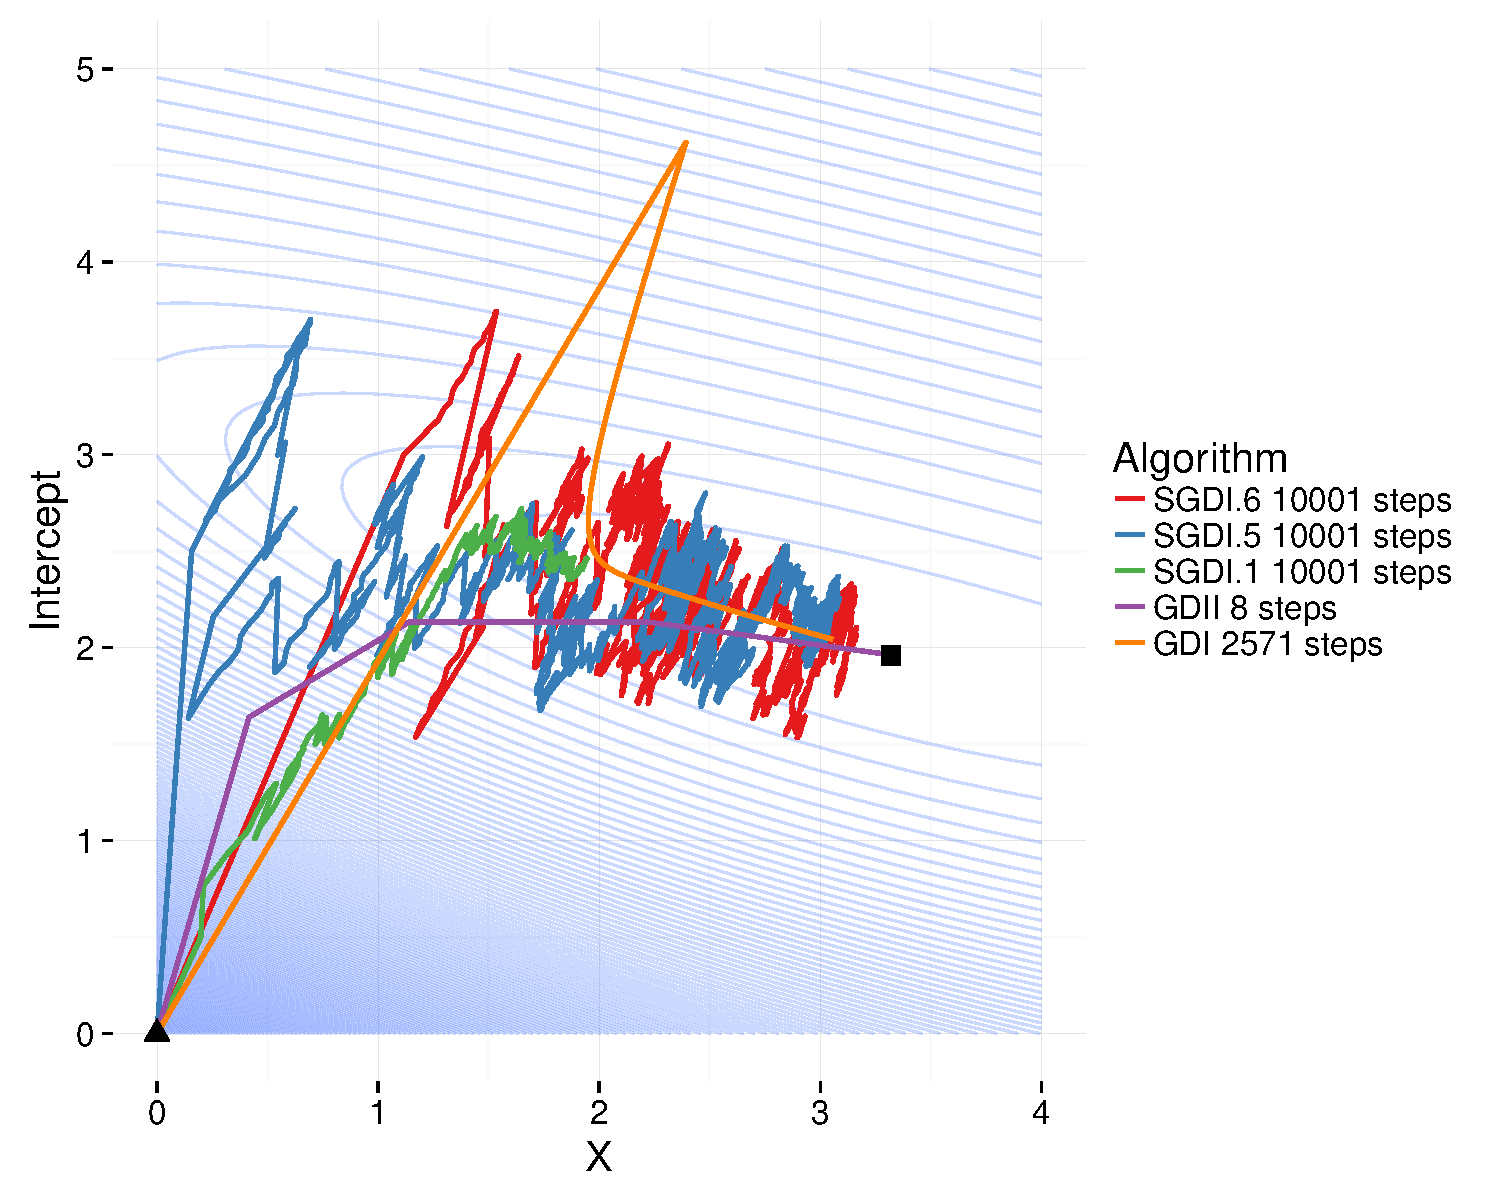
\includegraphics[width=\textwidth]{Obrazki/Numeryka/contour_00.pdf}
     \caption{$\beta_0 = (0,0)$}
   \end{subfigure}
   \begin{subfigure}[h!]{0.49\textwidth}
   %     \centering
        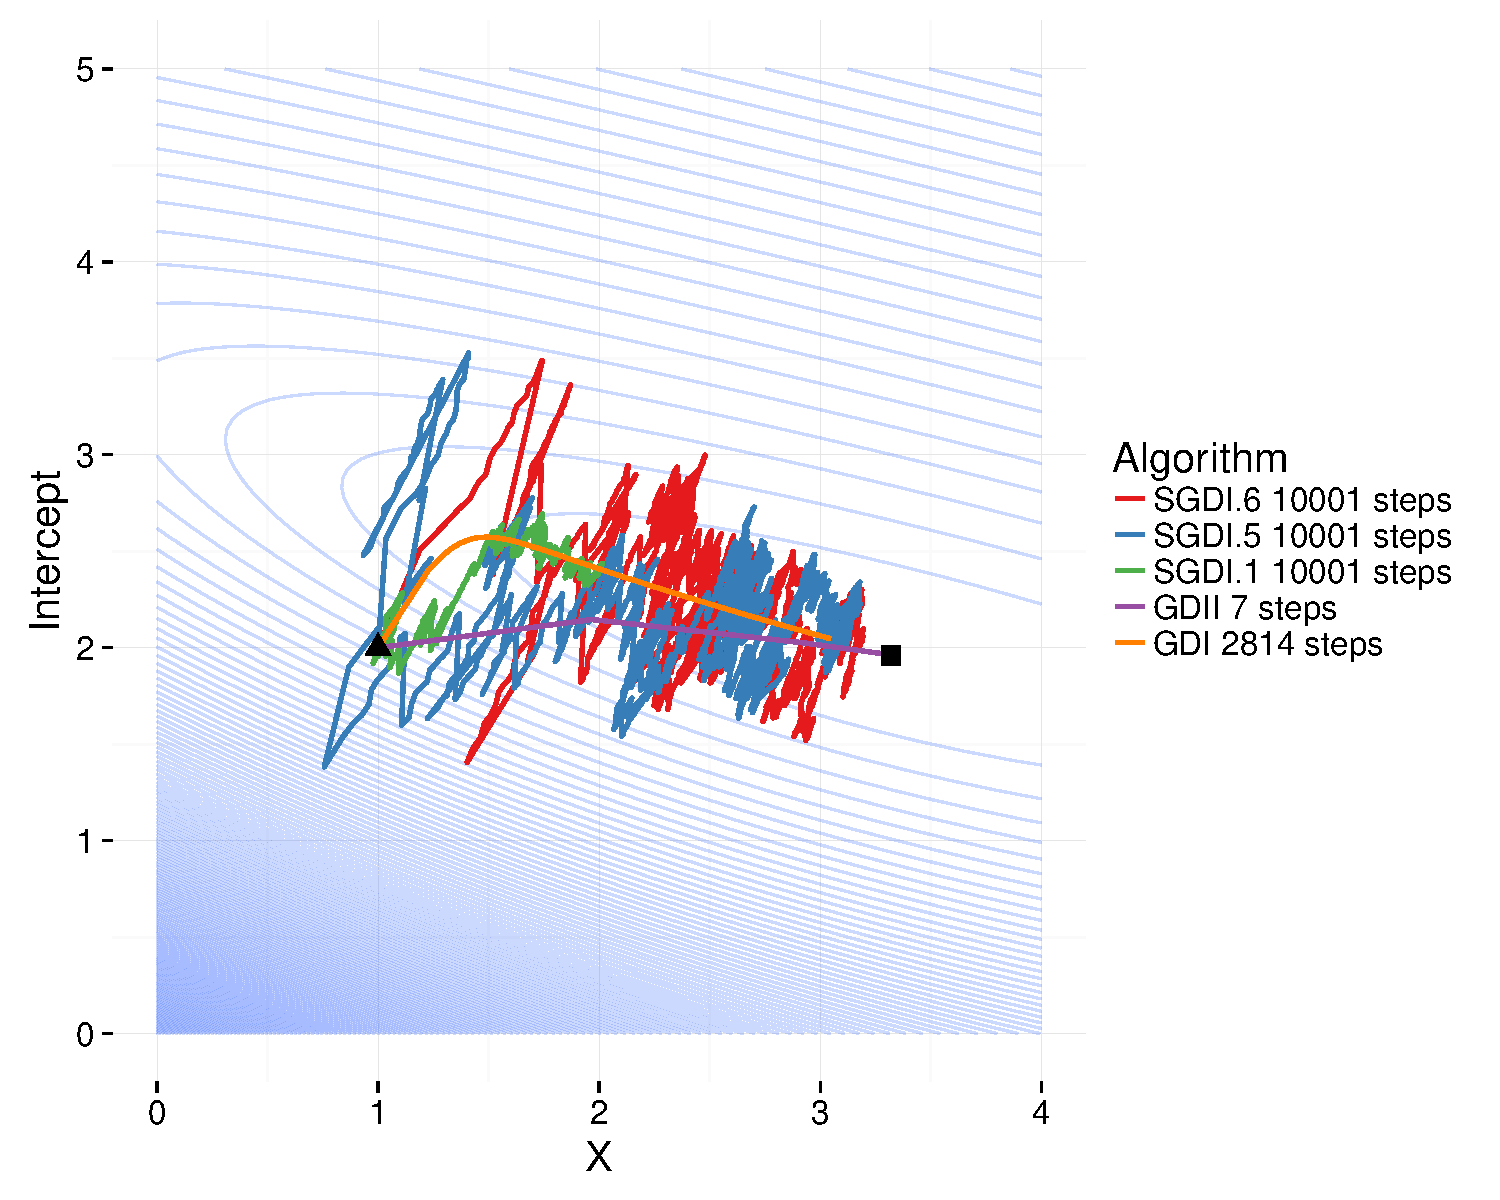
\includegraphics[width=\textwidth]{Obrazki/Numeryka/contour_2_1.pdf}
        \caption{$\beta_0 = (1,2)$}
      \end{subfigure}
   \begin{subfigure}[h!]{0.49\textwidth}
      %     \centering
           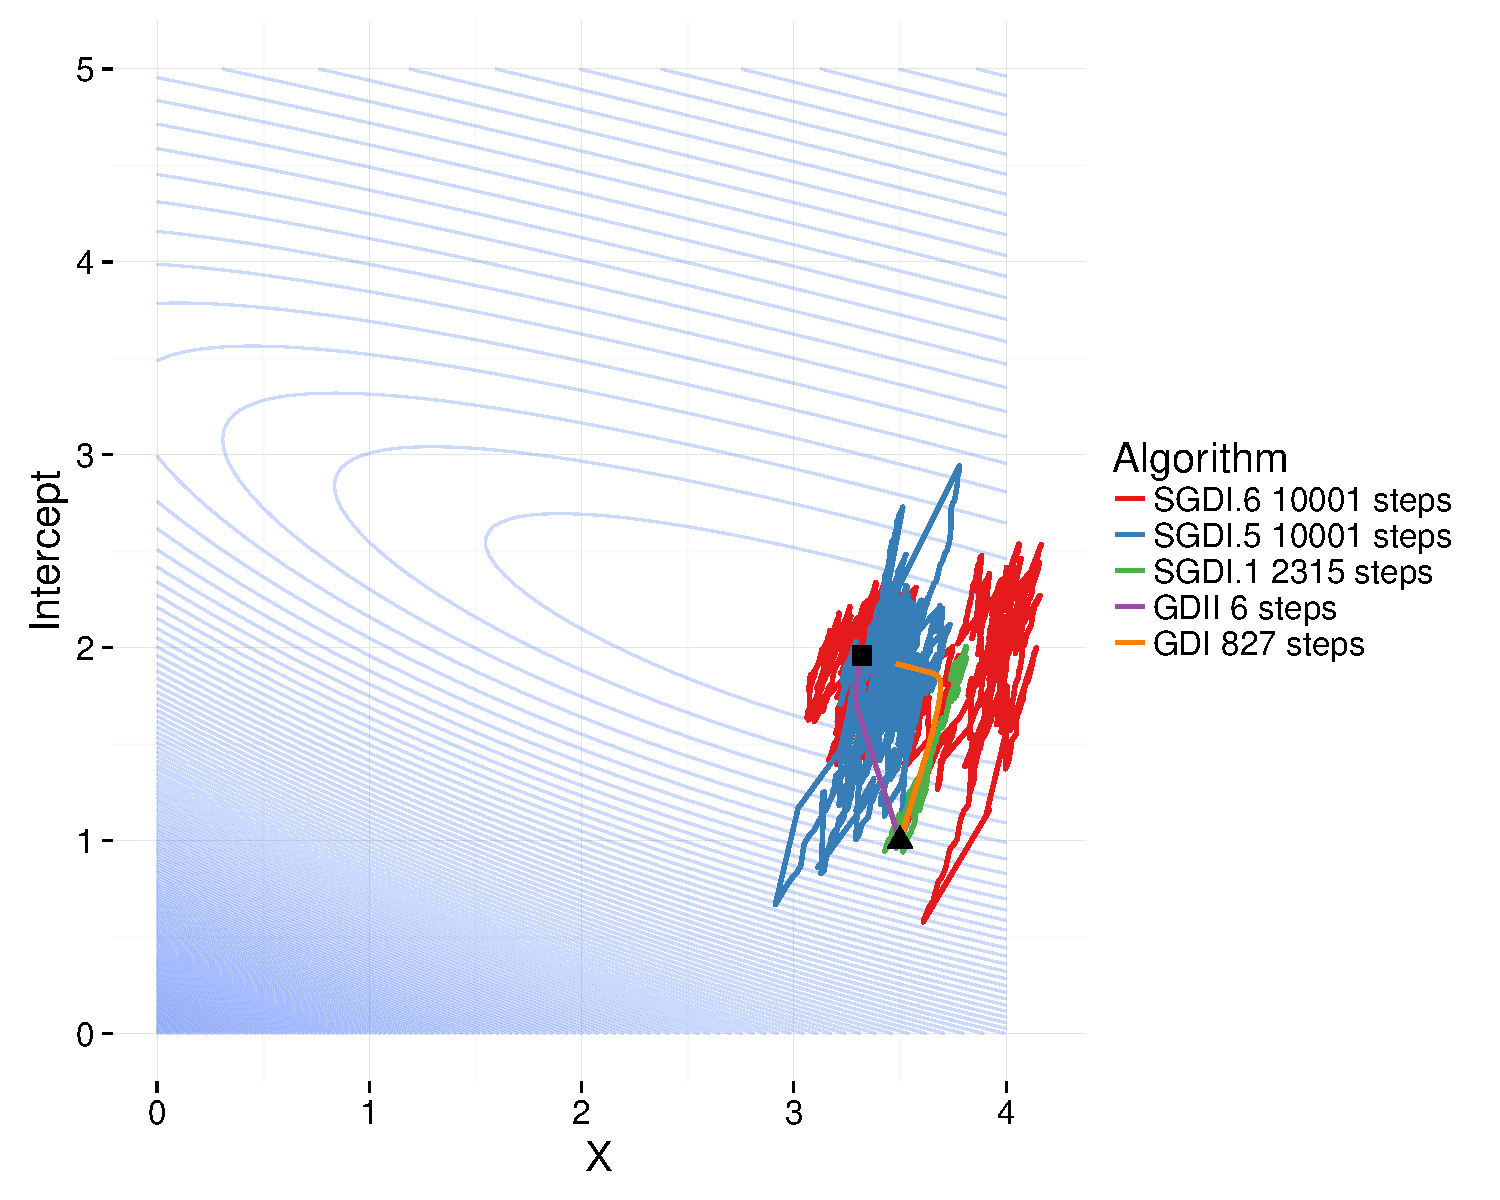
\includegraphics[width=\textwidth]{Obrazki/Numeryka/contour_35_1.pdf}
           \caption{$\beta_0 = (3.5,1)$}
                 \end{subfigure}
   \begin{subfigure}[h!]{0.49\textwidth}
         %     \centering
              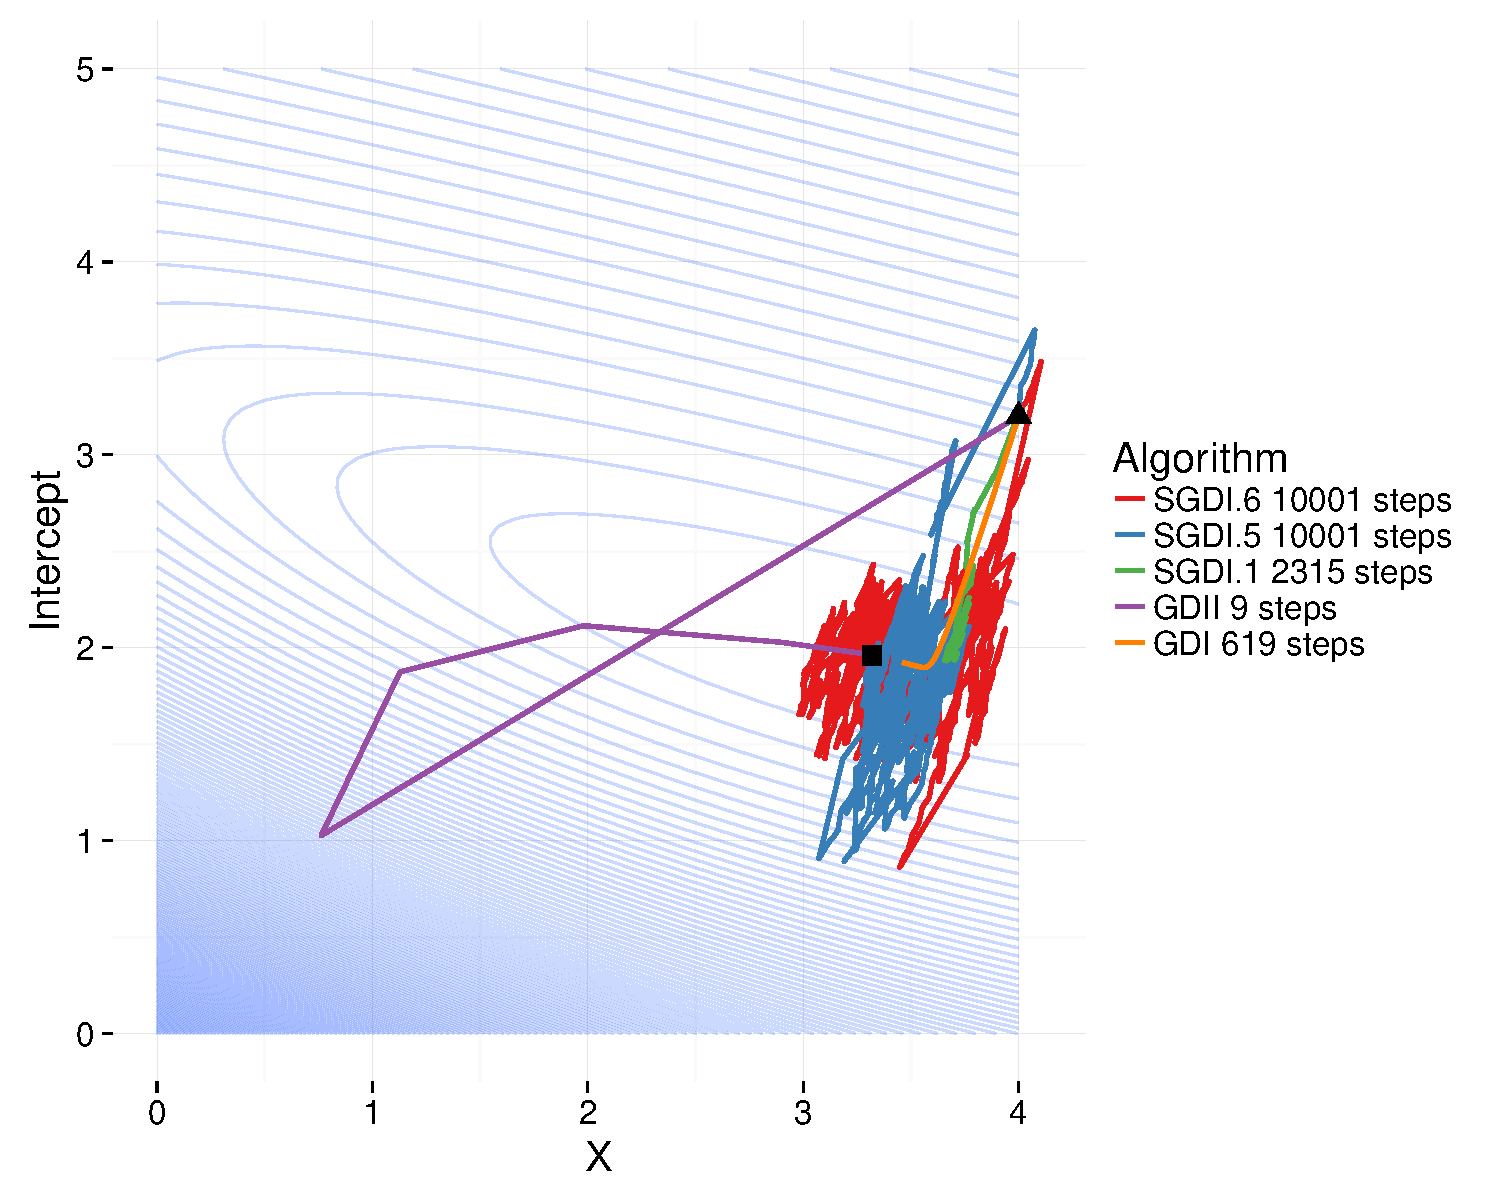
\includegraphics[width=\textwidth]{Obrazki/Numeryka/contour_4_32.pdf}
              \caption{$\beta_0 = (4,3.2)$}
            \end{subfigure}
\end{center}
\caption{\label{fig:sc5asd} Porównanie algorytmów spadku gradientu w modelu regresji logistycznej. Wykresy przedstawiają ścieżki zbieżności w kolejnych krokach algorytmów spadku gradientu. Ustalono maksymalną liczbę iteracji na 10001, zaś warunek stopu ustalono na $\varepsilon=10^{-5}$. Trójkątem zaznaczono punkt startowy, a~kwadratem wyestymowane rozwiązanie przy pomocy funkcji \texttt{glm()}. Przez \texttt{GDI} oznaczono algorytmu spadku gradientu rzędu I, zaś przez \texttt{GDII} rzędu II. Oznaczenie \texttt{SGD.i} odpowiada 3 algorytmom stochastycznego spadku gradientu o~różnych ciągach odpowiedzialnych za długość kroku. Indeks $i$ odpowiada ciągowi wybranemu na zasadzie $\alpha_{k,i} = i/\sqrt{k}$. Ziarno losowania ustalono na 4561.}
\end{figure}

Na wykresach na Rysunkach \ref{fig:scasd} - \ref{fig:sc4asd} osie dopasowane są do obecnej symulacji. 

\newpage

\begin{figure}[hbt!]
  %\vspace{-10pt}
  \begin{center}
   \begin{subfigure}[h!]{0.99\textwidth}
      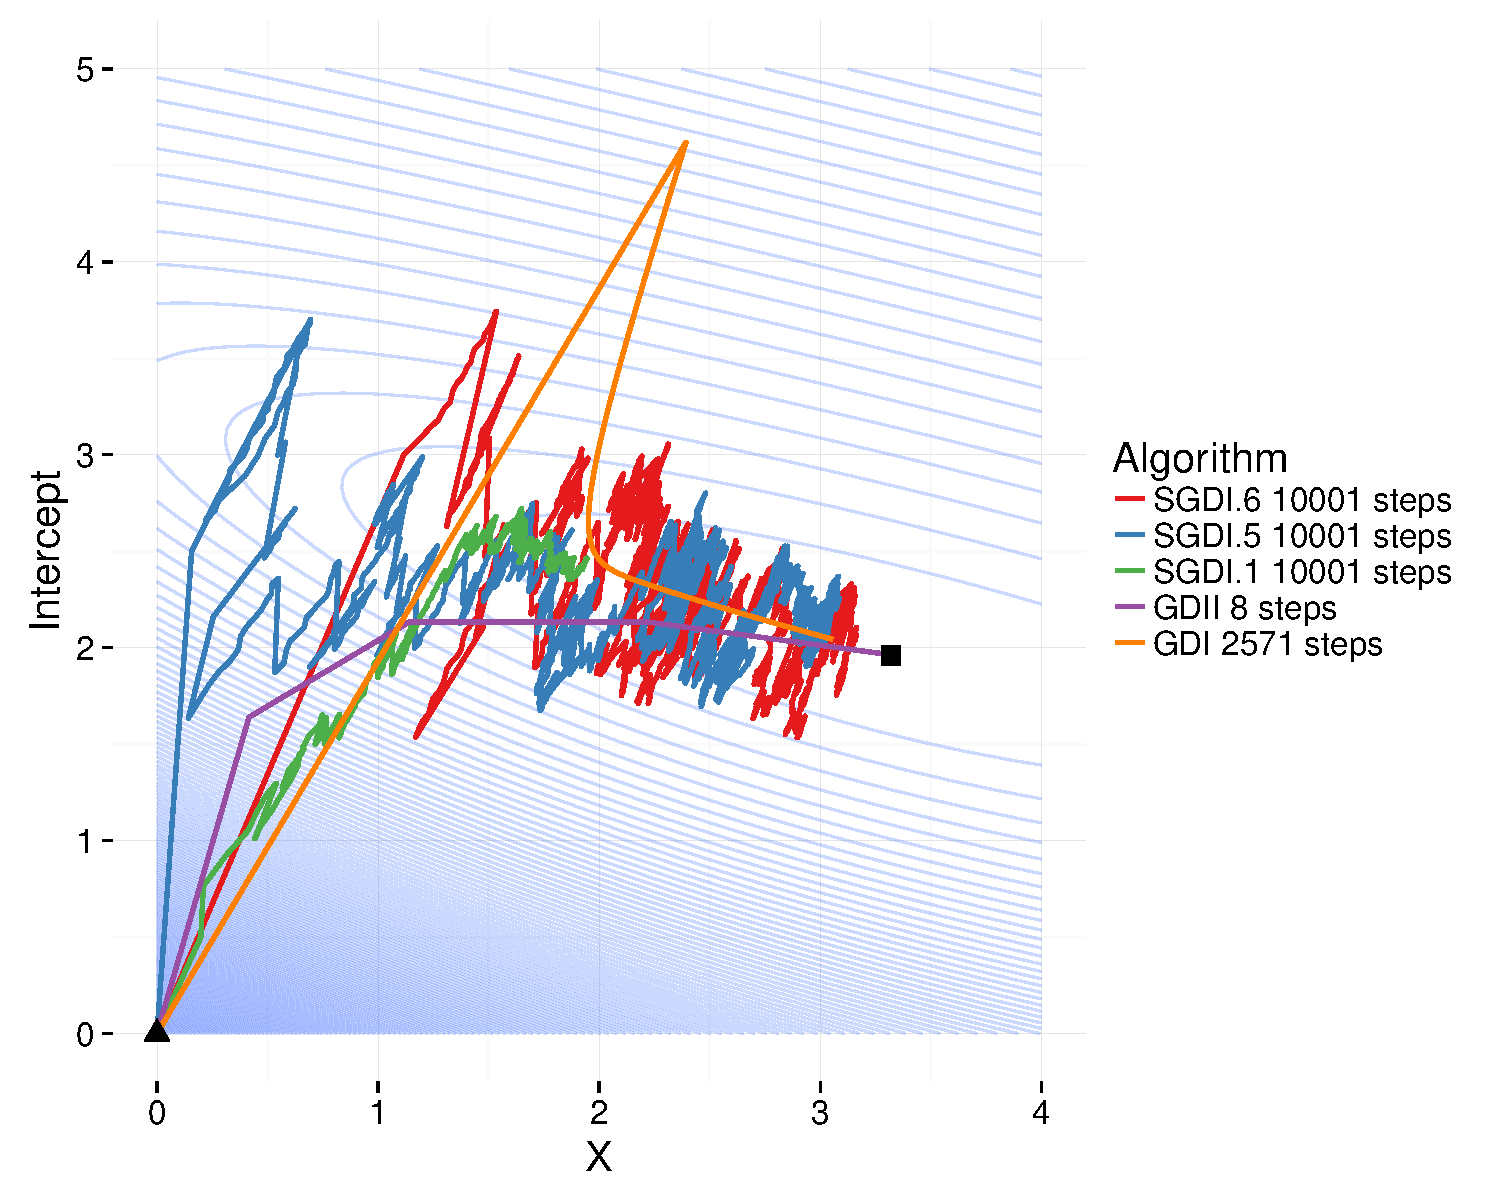
\includegraphics[width=\textwidth, height=270pt]{Obrazki/Numeryka/sgd_00_1.pdf}
      \caption{$\beta_0 = (0,0)$, ziarno losowania: 4561.}
   \end{subfigure}     
   \begin{subfigure}[h!]{0.99\textwidth}
      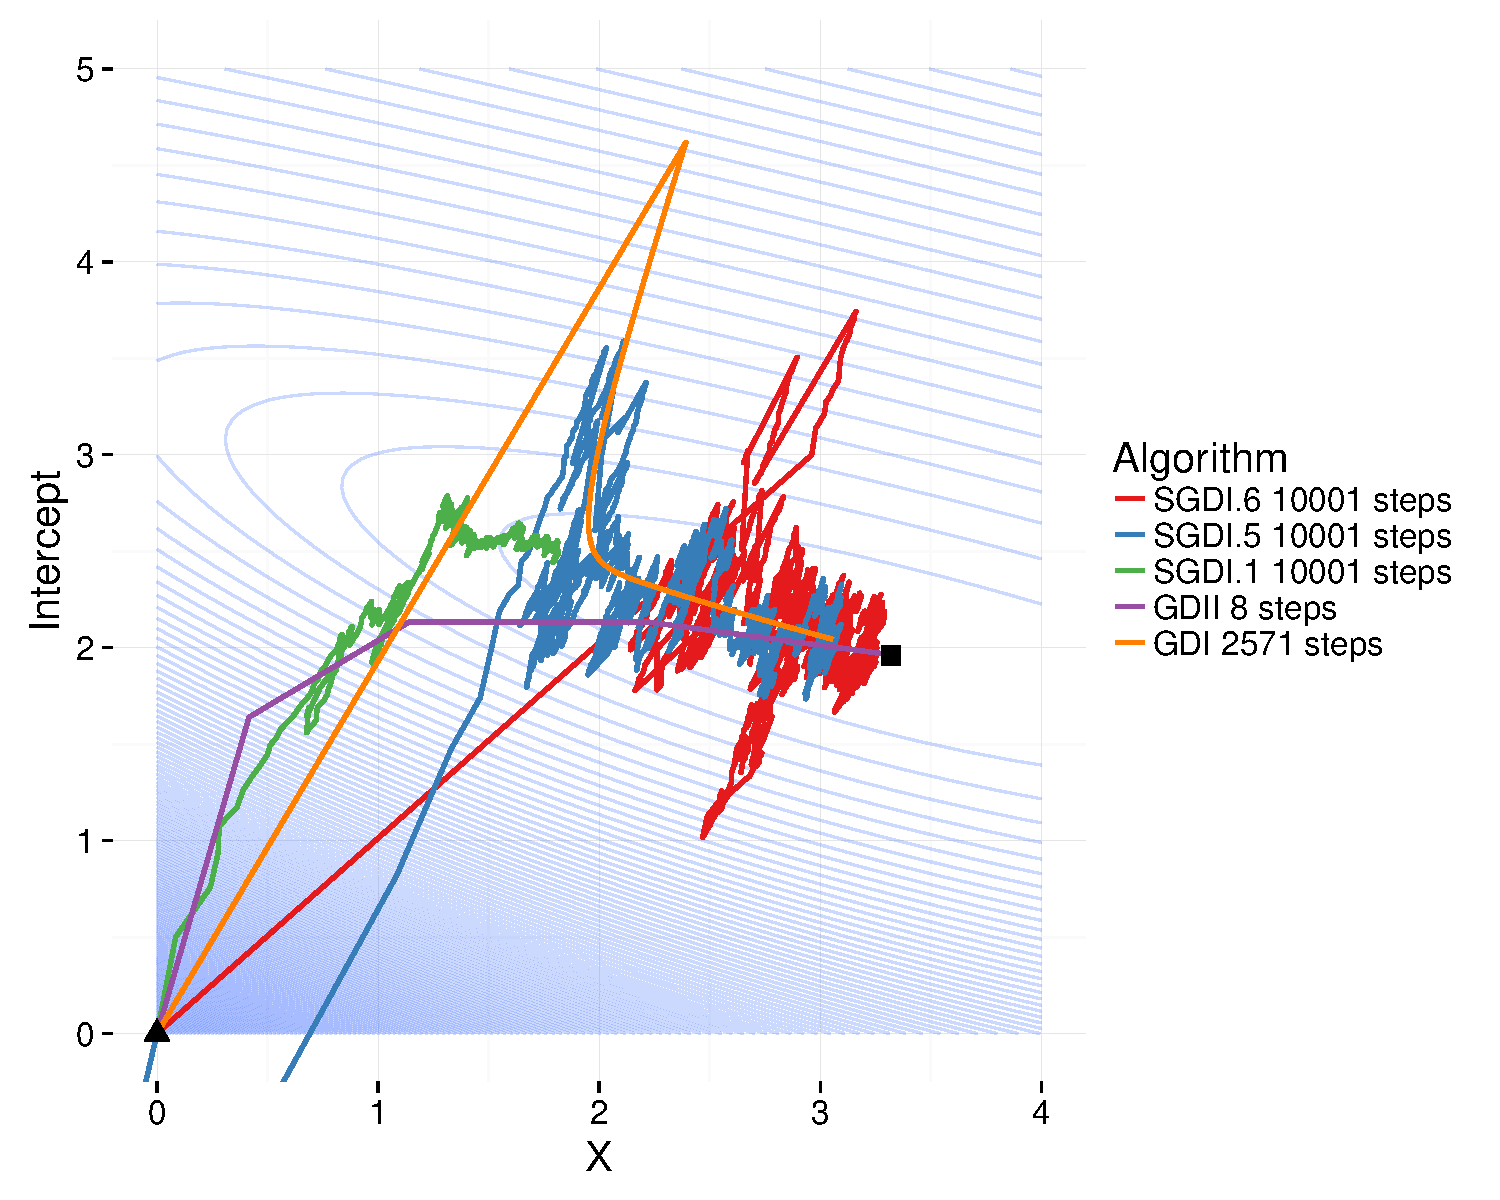
\includegraphics[width=\textwidth, height=270pt]{Obrazki/Numeryka/sgd_00_2.pdf}
      \caption{$\beta_0 = (0,0)$, ziarno losowania: 456.}
   \end{subfigure}  \end{center}
  %\vspace{-10pt}
  \caption[Porównanie algorytmów spadku gradientu dla punktu startowego $\beta_0 = (0,0)$.]{\label{fig:scasd}Porównanie algorytmów spadku gradientu w modelu regresji logistycznej. Wykresy przedstawiają ścieżki zbieżności w kolejnych krokach algorytmów spadku gradientu. Ustalono maksymalną liczbę iteracji na 10001, zaś warunek stopu na $\varepsilon=10^{-5}$. Trójkątem zaznaczono punkt startowy, a~kwadratem wyestymowane rozwiązanie przy pomocy funkcji \texttt{glm()}. Przez \texttt{GDI} oznaczono algorytmu spadku gradientu rzędu I, zaś przez \texttt{GDII} rzędu II. Oznaczenie \texttt{SGD.i} odpowiada 3 algorytmom stochastycznego spadku gradientu o~różnych ciągach odpowiedzialnych za długość kroku. Indeks $i$ odpowiada ciągowi wybranemu na zasadzie $\alpha_{k,i} = i/\sqrt{k}$. Punkt startowy $\beta_0 = (0,0)$.}
\end{figure}


\begin{figure}[hbt!]
  %\vspace{-10pt}
  \begin{center}
   \begin{subfigure}[h!]{0.9\textwidth}
      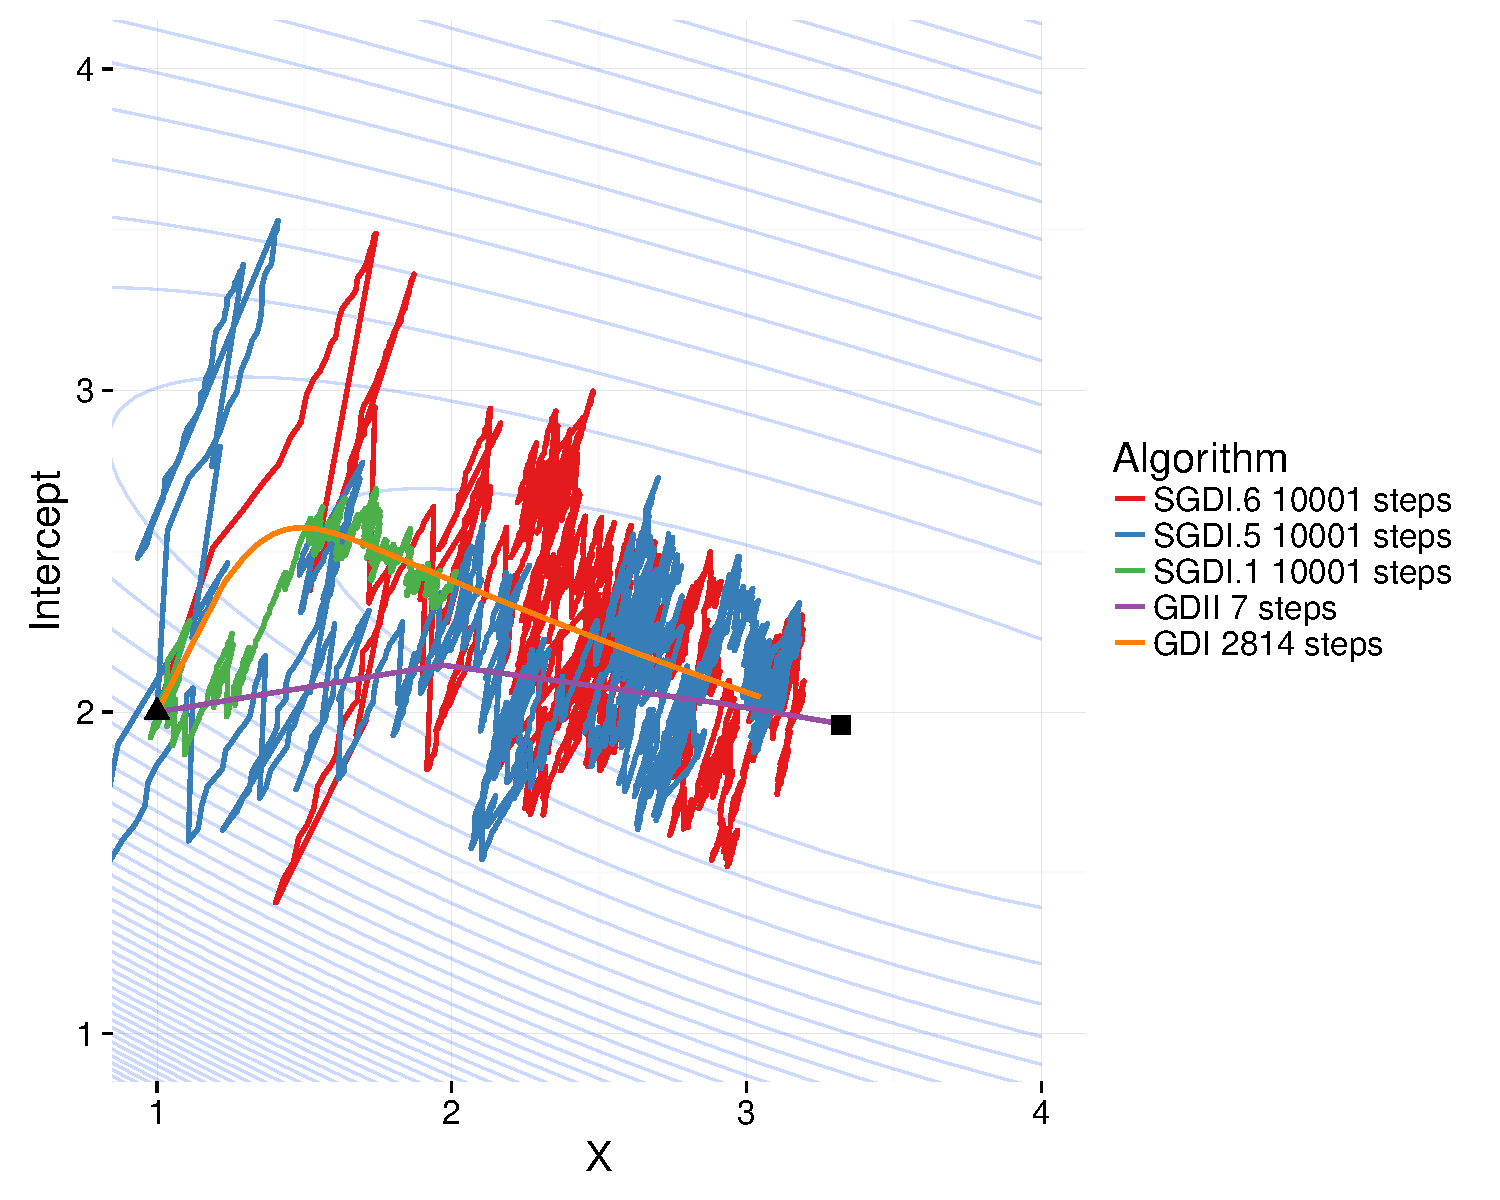
\includegraphics[width=\textwidth, height=270pt]{Obrazki/Numeryka/sgd_1_2_1.pdf}
      \caption{$\beta_0 = (1,2)$, ziarno losowania: 4561.}
   \end{subfigure}     
   \begin{subfigure}[h!]{0.9\textwidth}
      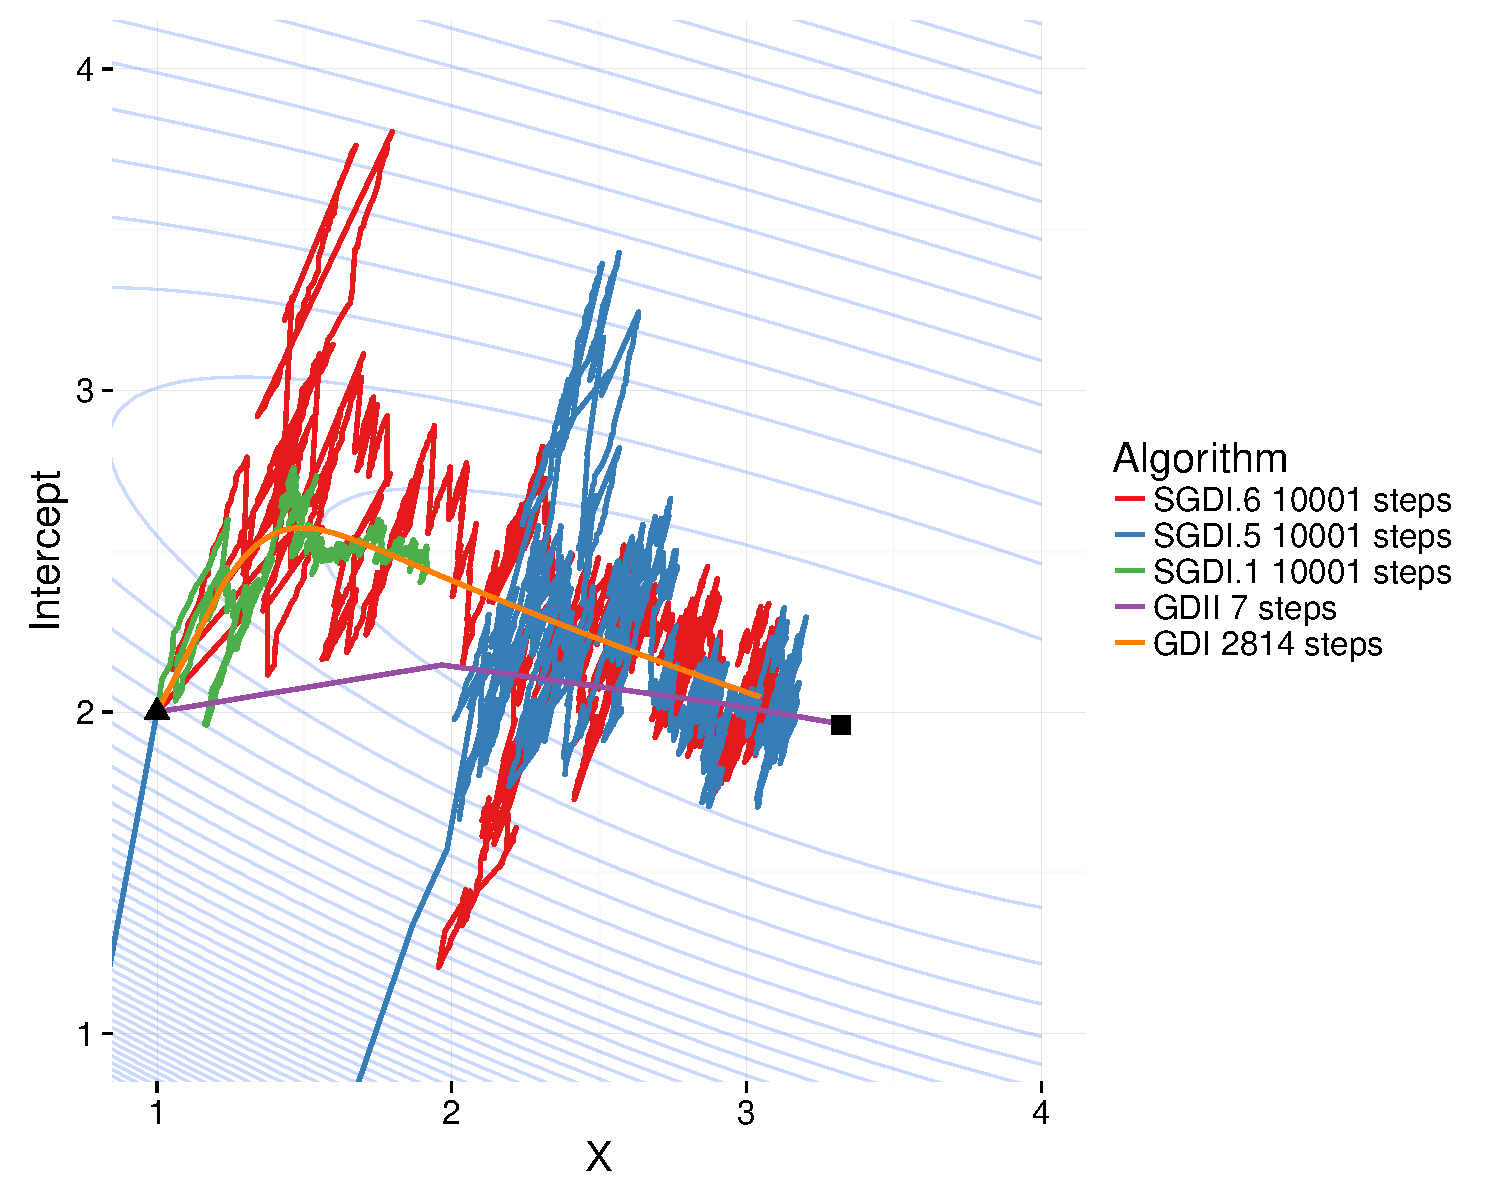
\includegraphics[width=\textwidth, height=270pt]{Obrazki/Numeryka/sgd_1_2_2.pdf}
      \caption{$\beta_0 = (1,2)$, ziarno losowania: 456.}
   \end{subfigure}  \end{center}
  %\vspace{-10pt}
  \caption[Porównanie algorytmów spadku gradientu dla punktu startowego $\beta_0 = (1,2)$.]{\label{fig:sc2asd}Porównanie algorytmów spadku gradientu w modelu regresji logistycznej. Wykresy przedstawiają ścieżki zbieżności w kolejnych krokach algorytmów spadku gradientu. Ustalono maksymalną liczbę iteracji na 10001, zaś warunek stopu na $\varepsilon=10^{-5}$. Trójkątem zaznaczono punkt startowy, a~kwadratem wyestymowane rozwiązanie przy pomocy funkcji \texttt{glm()}. Przez \texttt{GDI} oznaczono algorytmu spadku gradientu rzędu I, zaś przez \texttt{GDII} rzędu II. Oznaczenie \texttt{SGD.i} odpowiada 3 algorytmom stochastycznego spadku gradientu o~różnych ciągach odpowiedzialnych za długość kroku. Indeks $i$ odpowiada ciągowi wybranemu na zasadzie $\alpha_{k,i} = i/\sqrt{k}$. Punkt startowy $\beta_0 = (1,2)$.}
\end{figure}


\begin{figure}[hbt!]
  %\vspace{-10pt}
  \begin{center}
   \begin{subfigure}[h!]{0.9\textwidth}
      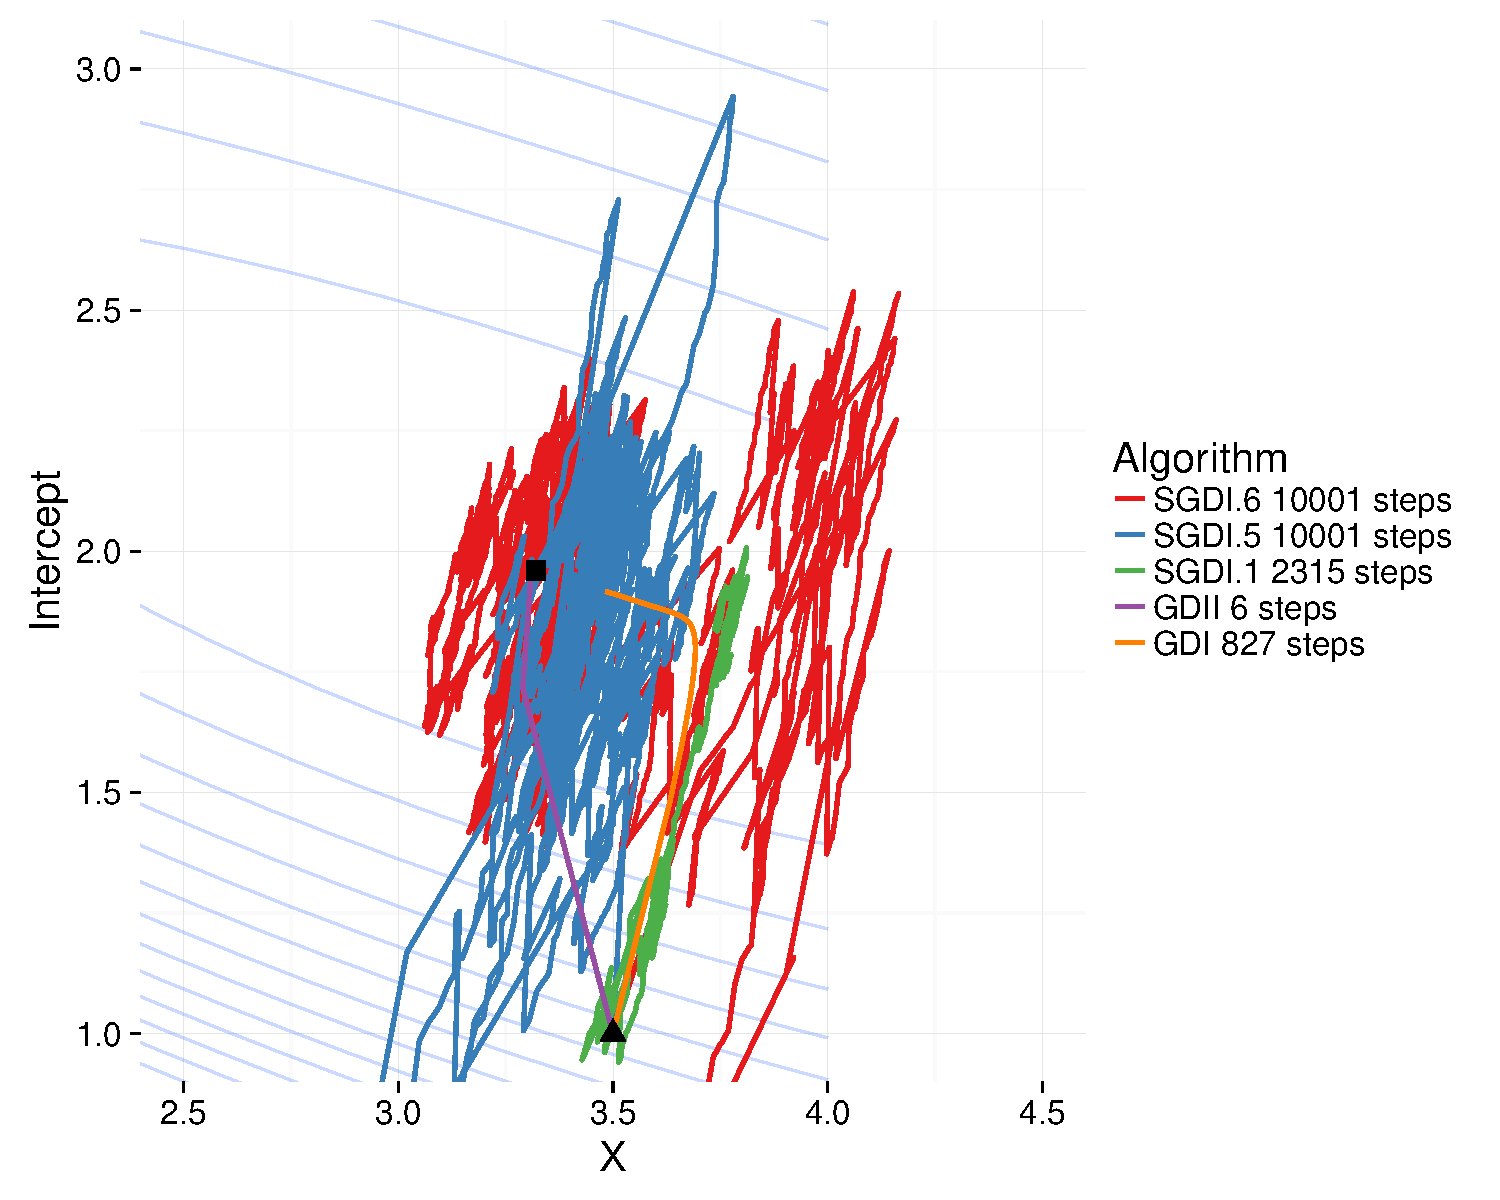
\includegraphics[width=\textwidth, height=270pt]{Obrazki/Numeryka/sgd_35_1_1.pdf}
      \caption{$\beta_0 = (3.5,1)$, ziarno losowania: 4561.}
   \end{subfigure}     
   \begin{subfigure}[h!]{0.9\textwidth}
      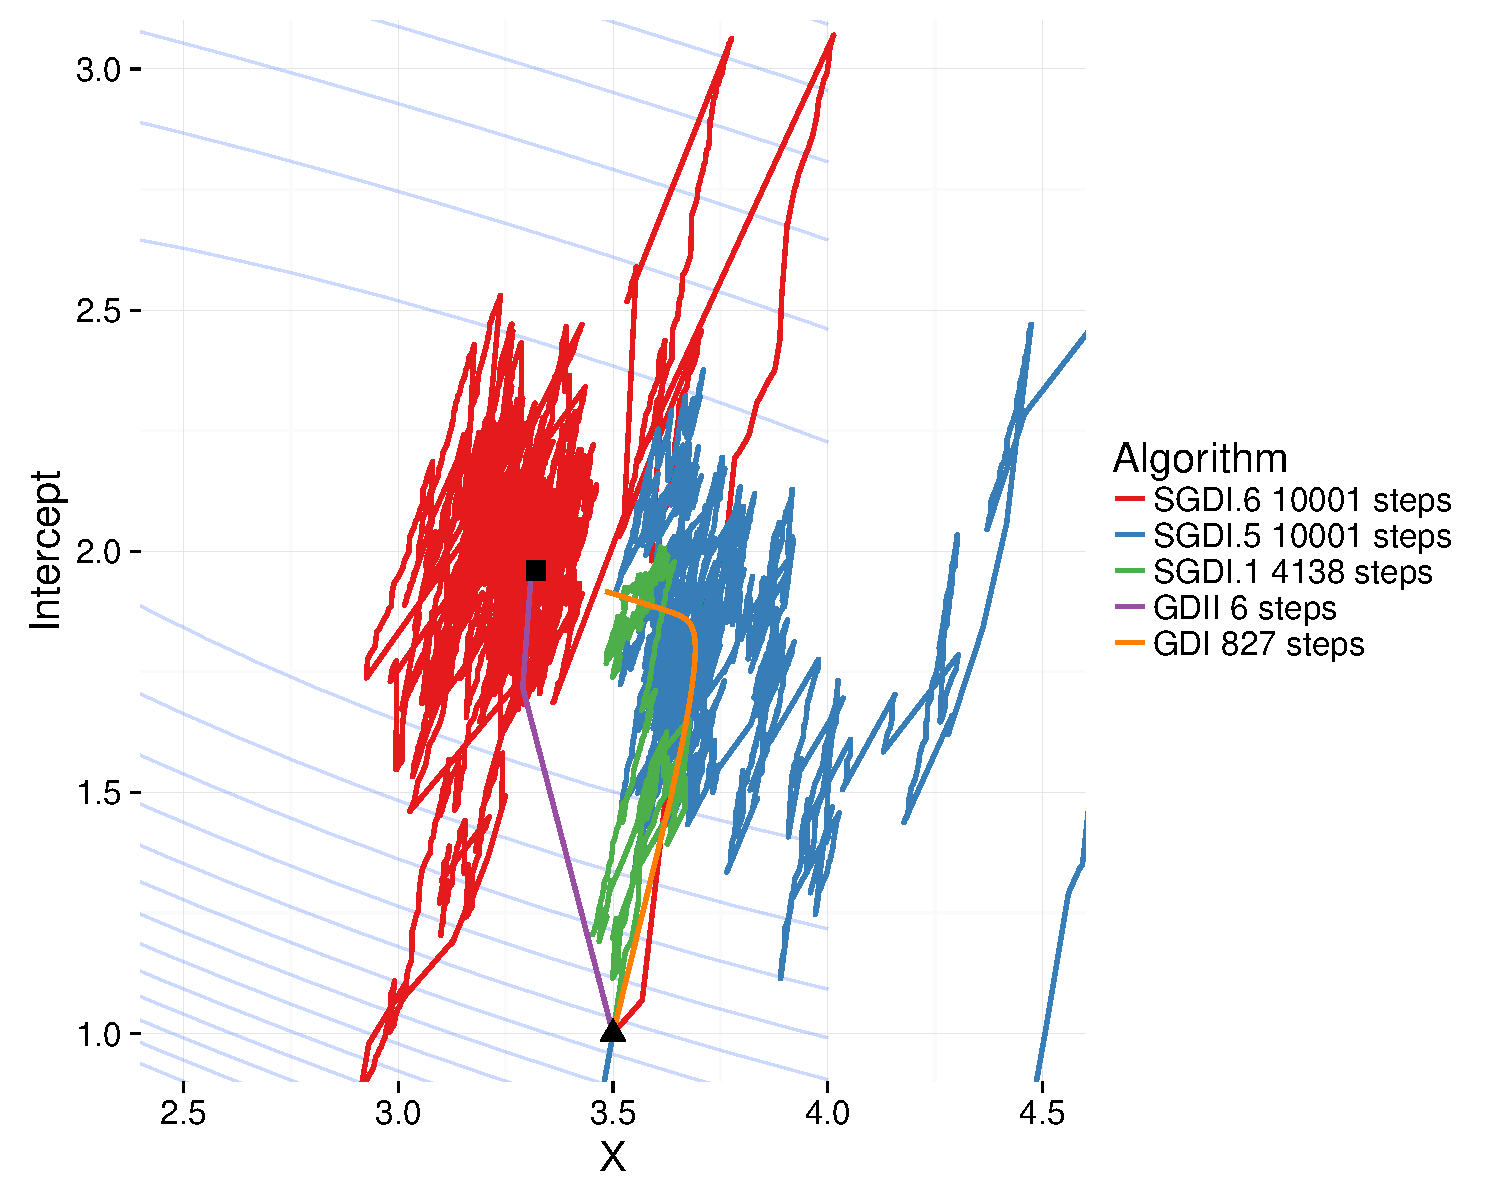
\includegraphics[width=\textwidth, height=270pt]{Obrazki/Numeryka/sgd_35_1_2.pdf}
      \caption{$\beta_0 = (3.5,1)$, ziarno losowania: 456.}
   \end{subfigure}  \end{center}
  %\vspace{-10pt}
  \caption[Porównanie algorytmów spadku gradientu dla punktu startowego $\beta_0 = (3.5,1)$.]{\label{fig:sc3asd}Porównanie algorytmów spadku gradientu w modelu regresji logistycznej. Wykresy przedstawiają ścieżki zbieżności w kolejnych krokach algorytmów spadku gradientu. Ustalono maksymalną liczbę iteracji na 10001, zaś warunek stopu na $\varepsilon=10^{-5}$. Trójkątem zaznaczono punkt startowy, a~kwadratem wyestymowane rozwiązanie przy pomocy funkcji \texttt{glm()}. Przez \texttt{GDI} oznaczono algorytmu spadku gradientu rzędu I, zaś przez \texttt{GDII} rzędu II. Oznaczenie \texttt{SGD.i} odpowiada 3 algorytmom stochastycznego spadku gradientu o~różnych ciągach odpowiedzialnych za długość kroku. Indeks $i$ odpowiada ciągowi wybranemu na zasadzie $\alpha_{k,i} = i/\sqrt{k}$. Punkt startowy $\beta_0 = (3.5,1)$.}
\end{figure}


\begin{figure}[hbt!]
  %\vspace{-10pt}
  \begin{center}
   \begin{subfigure}[h!]{0.9\textwidth}
      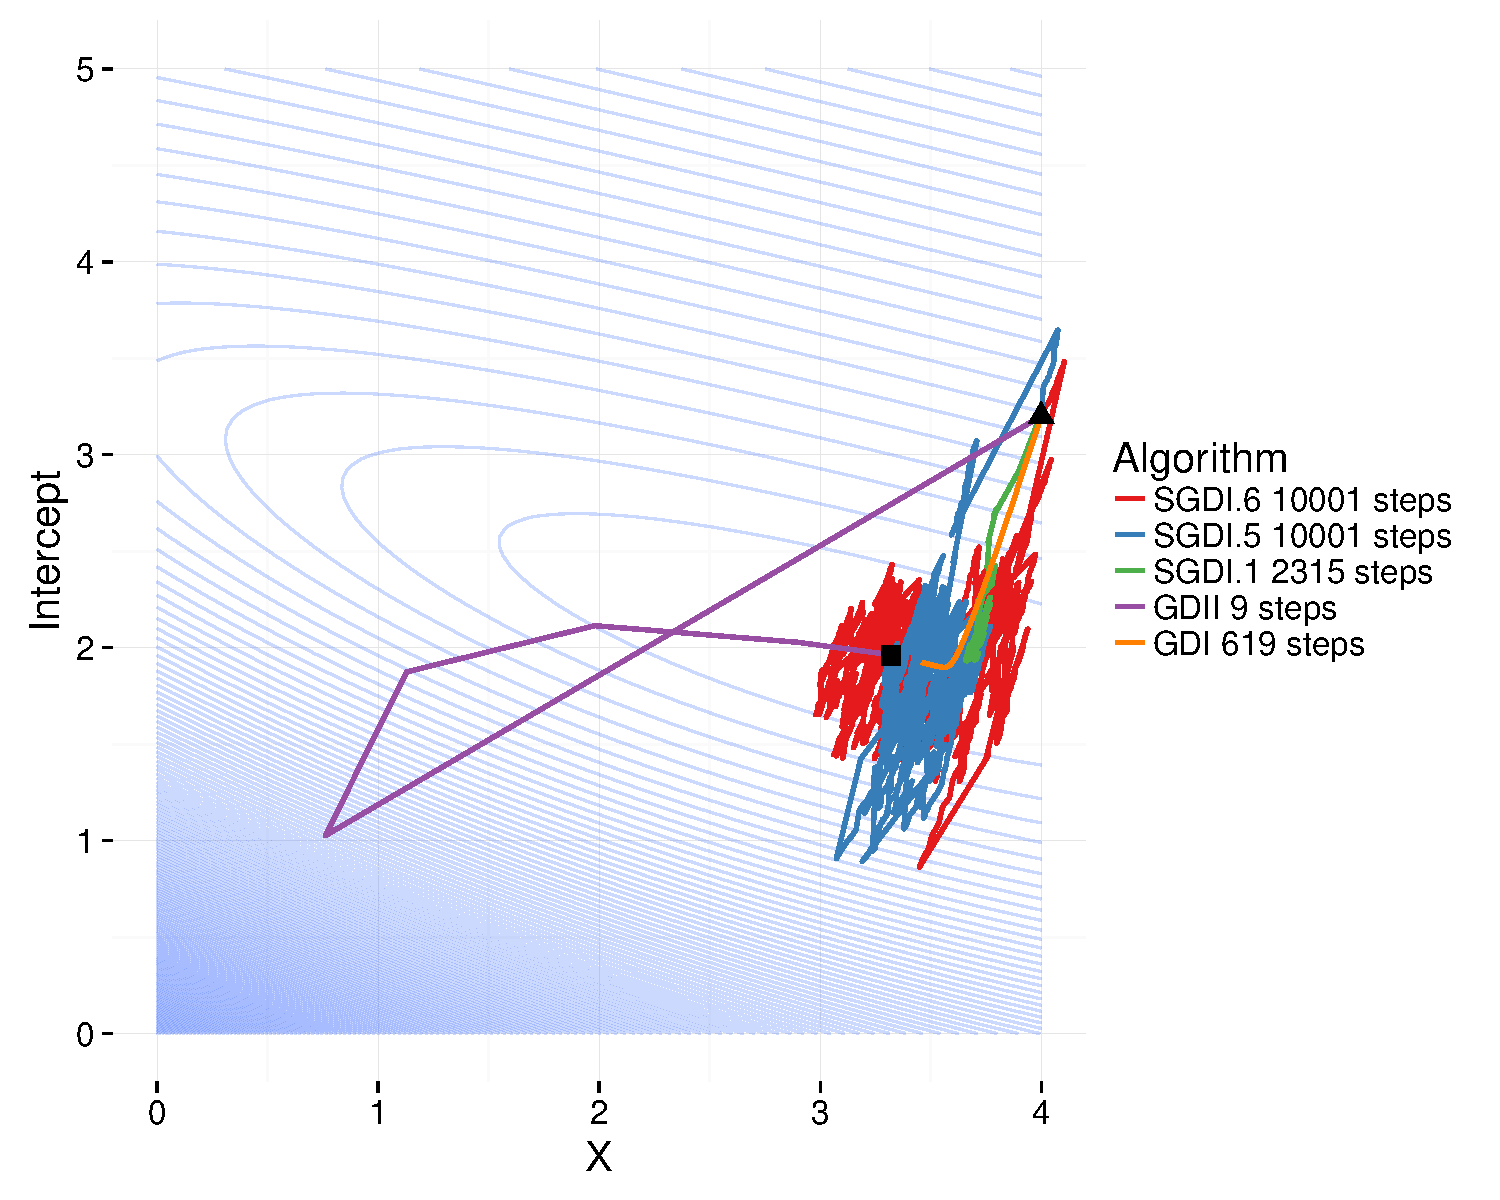
\includegraphics[width=\textwidth, height=270pt]{Obrazki/Numeryka/sgd_32_4_1.pdf}
      \caption{$\beta_0 = (4,3.2)$, ziarno losowania: 4561.}
   \end{subfigure}     
   \begin{subfigure}[h!]{0.9\textwidth}
      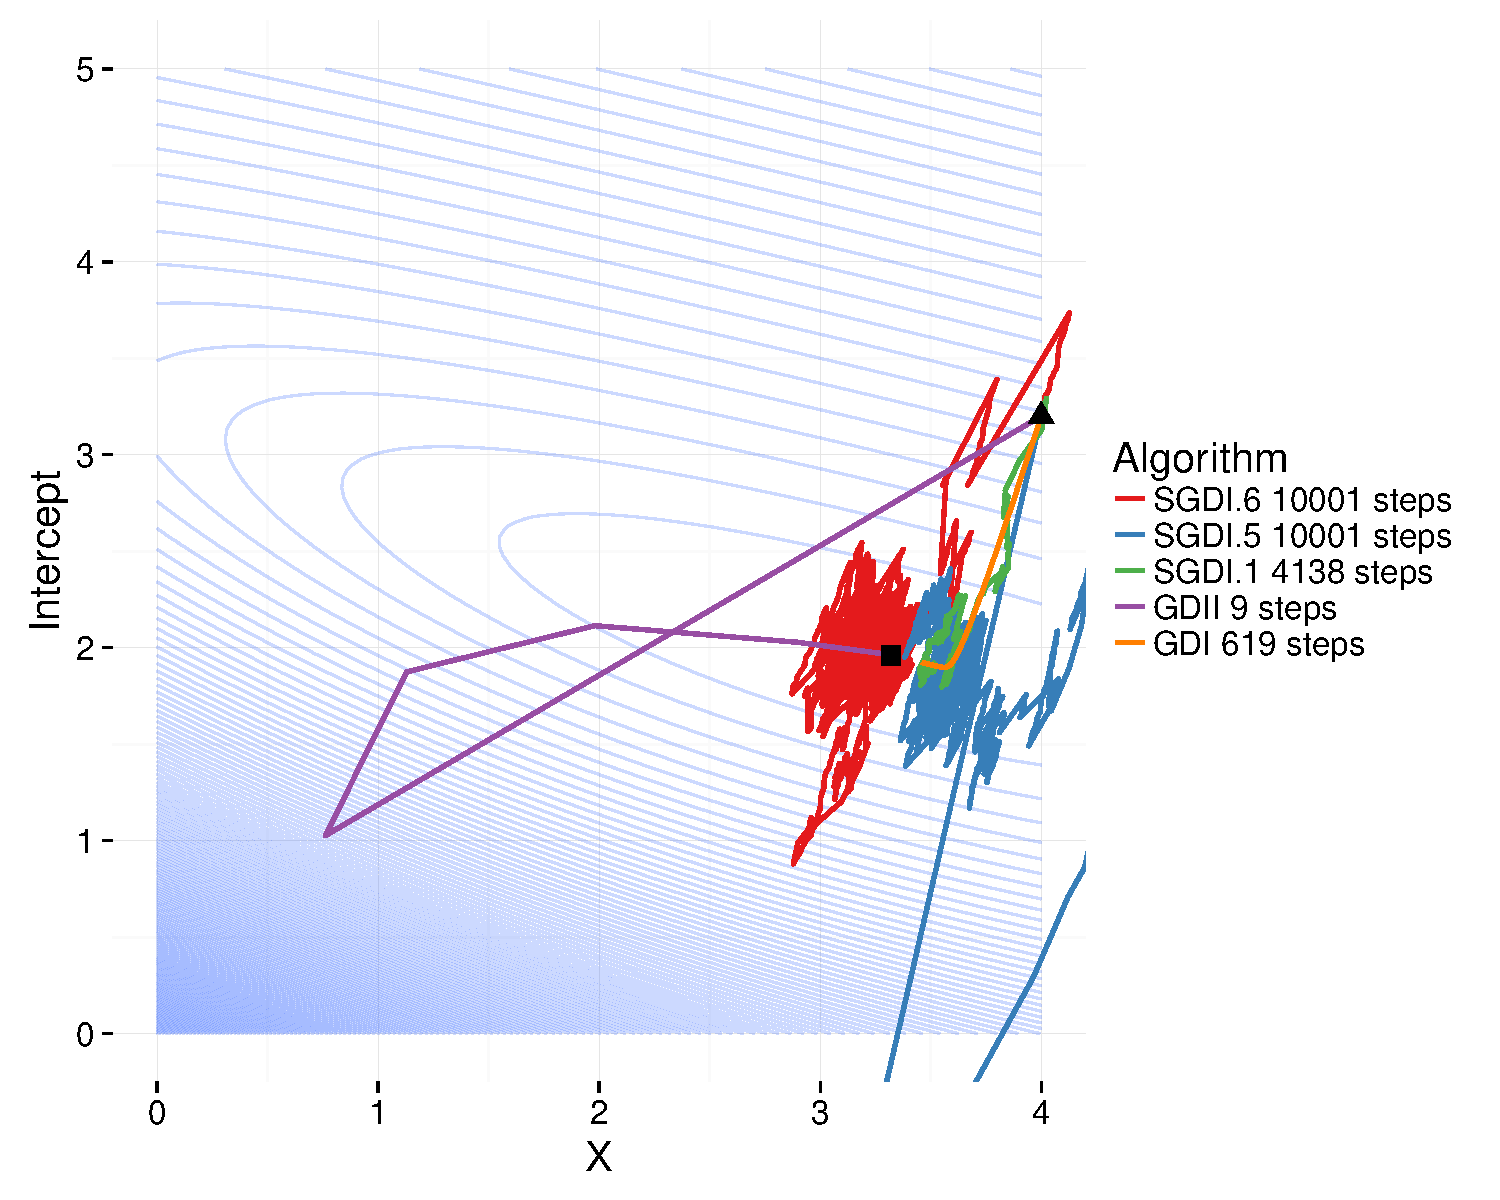
\includegraphics[width=\textwidth, height=270pt]{Obrazki/Numeryka/sgd_32_4_2.pdf}
      \caption{$\beta_0 = (4,3.2)$, ziarno losowania: 456.}
   \end{subfigure}  \end{center}
  %\vspace{-10pt}
  \caption[Porównanie algorytmów spadku gradientu dla punktu startowego $\beta_0 = (4,3.2)$.]{\label{fig:sc4asd}Porównanie algorytmów spadku gradientu w modelu regresji logistycznej. Wykresy przedstawiają ścieżki zbieżności w kolejnych krokach algorytmów spadku gradientu. Ustalono maksymalną liczbę iteracji na 10001, zaś warunek stopu na $\varepsilon=10^{-5}$. Trójkątem zaznaczono punkt startowy, a~kwadratem wyestymowane rozwiązanie przy pomocy funkcji \texttt{glm()}. Przez \texttt{GDI} oznaczono algorytmu spadku gradientu rzędu I, zaś przez \texttt{GDII} rzędu II. Oznaczenie \texttt{SGD.i} odpowiada 3 algorytmom stochastycznego spadku gradientu o~różnych ciągach odpowiedzialnych za długość kroku. Indeks $i$ odpowiada ciągowi wybranemu na zasadzie $\alpha_{k,i} = i/\sqrt{k}$. Punkt startowy $\beta_0 = (4,3.2)$.}
\end{figure}


\newpage

\subsubsection{Podsumowanie symulacji}
W trackie symulacji badano zachowanie trajektorii zbieżności w kolejnych krokach algorytmów spadku gradientu. Algorytm spadku gradientu rzędu II zbiegał do rozwiązania wyznaczonego przez funkcję \texttt{glm()} i osiągał zbieżność po najmniejszej liczbie kroków, jednak należy pamiętać o kosztownych obliczeniowo operacjach odwracania macierzy Hesjanu wykonywanych w trakcie optymalizacji z wykorzystaniem tej metody. 

Algorytm spadku gradientu rzędu I zbiegał do rozwiązania wyznaczonego przez funkcję \texttt{glm()} w sytuacjach, gdy warunek stopu był dostatecznie mały ($\varepsilon = 10^{-5}$, Rysunek \ref{fig:scasd}). Znajdywał się również w okolicach bliskich rozwiązania (Rysunki \ref{fig:sc2asd} - \ref{fig:sc4asd}), jednak nie osiągnął równie bliskich punktów co algorytm spadku gradientu rzędu II, z racji na zbyt duży warunek stopu. Gdy punkt startowy był bliski rozwiązaniu pochodzącemu z funkcji \texttt{glm()} algorytm spadku gradientu rzędu I miał początkowo problem z obraniem właściwego toru zbieżności i~ostatecznie wypadł najgorzej ze wszystkich sprawdzanych metod. Estymacja w algorytmie spadku gradientu rzędu I miała mniej kroków niż w algorytmie stochastycznego spadku gradientu, co może wynikać z mało różnowartościowych wartości optymalizowanej funkcji log-wiarogodności w badanym obszarze, będącym stosunkowo blisko rozwiązania.

W przypadku stochastycznego spadku gradientu widać duże wahania w trajektoriach zbieżności algorytmu. W ramach symulacji badano wiele ciągów odpowiadających za długość kroku w~tym algorytmie i~ostatecznie zdecydowano na ukazanie w pracy tych, dzięki którym osiągana zbieżność dotyczyła największej liczby punktów startowych. Algorytm \texttt{SGDI.1} w~każdym z~możliwych przypadków miał zbyt małe wartości ciągu odpowiadającego za długości kroków, przez co nie osiągał punktu wyliczonego przez funkcję \texttt{glm()}. \texttt{SGDI.1} ukazano aby uświadomić jak ważnym aspektem jest odpowiednie dobranie długości kroków. Dla odpowiednio dobranego ciągu długości kroków o dużych wartościach, jakim był ciąg $\alpha_{ki} = i/\sqrt{k}, i = 5, 6$, w~wielu sytuacjach doszło do zbieżności w tym samym punkcie, w którym zbiegł algorytm zaimplementowany w \texttt{glm()}. Najlepiej widać to na Rysunkach \ref{fig:scasd} i \ref{fig:sc2asd} (gdzie w zbieżności algorytmu przeszkodził zbyt duży warunek stopu). Ciekawy rezultat osiągnięto na Rysunku \ref{fig:sc3asd}, gdzie osiągnięto zbieżność do punktu bliskiego wyliczonemu przez funkcję \texttt{glm()}, a algorytm po wkroczeniu do ostatniej widocznej warstwicy już poza nią nie wykraczał. 

Istota losowości odgrywa kluczową rolę w algorytmie stochastycznego spadku gradientu i należy mieć świadomość, że przy różnych ziarnach losowości, a co za tymi idzie przy innej kolejności obserwacji, algorytm może zachowywać się odmiennie. 

Ostatecznie można stwierdzić, że w wielu przypadkach stochastyczny wariant optymalizacji funkcji log-wiarogodności w modelu regresji logistycznej daje zadowalające rezultaty, które są niekiedy podobne do tych osiągniętych dzięki algorytmom spadku gradientu. Dzieje się to jednak za sprawą właściwego wyboru ciągu odpowiadającego za długości poszczególnych kroków oraz przy odpowiednim warunku stopu algorytmu. Należy pamiętać, że jest to jednak algorytm stochastyczny i~istnieją nieliczne sytuacje, w~których osiągnięte dzięki niemu współczynniki są dalekie od prawdziwych.



%Na Rysunkach (\ref{fig:sc3asd}) i (\ref{fig:scasd}) widać, zwłaszcza dla Symulacji nr 2, że ścieżki wyznaczane przez algorytmy stochastycznego spadku gradientu nie pokrywają się ze ścieżką wyznaczoną przez algorytm spadku gradientu rzędu II, a raczej pokrywają się ze ścieżką algorytmu spadku gradientu rzędu I. W tych sytuacjach widać, że warianty stochastycznego spadku gradientu zmierzają bezpośrednio do rozwiązania w przypadkach gdy pierwsze kroki algorytmy są dłuższe, czyli gdy ustali się ciąg odpowiadający długościom kroków algorytmu na $\alpha_{ki} = \frac{i}{k}$ i $i>=4$.
%Rysunek (\ref{fig:sc4asd}) obrazuje ciekawy przypadek, w którym stochastyczne warianty algorytmów rozpoczynają estymację w kierunku przeciwnym do rzeczywistego optimum, by dopiero po kilku obserwacjach porzucić ten kierunek i szukać rozwiązania w okolicach zbliżonych do prawdziwego minimum. W tej sytuacji znowu widać, że im dłuższe proporcjonalnie kolejne kroki algorytmu, tym szanse na powrót na właściwe tory dla algorytmów stochastycznych jest większa. Algorytmy o indeksach $i = 1, 2$ nie posunęły się z optymalizacją za daleko od punktu startowego i nie zdążyły zawrócić na właściwy kierunek, zanim wyczerpały się wszystkie dostępne obserwacje. Najgorzej sprawuje się stochastyczny spadek gradientu na Rysunku (\ref{fig:sc2asd}), gdzie widać na powiększeniu, że algorytmy stochastyczne (a nawet spadek gradientu rzędu I) błądzą w kierunku jedynie zbliżonym do rzeczywistego kierunku, na którym znaleźć można optimum, jednak może to wynikać z małych różnic w wartości funkcji log-wiarogodności na obszarze błądzenia w poszukiwaniu minimum. Z Rysunku (\ref{fig:sc5asd}) można wywnioskować, że im dłuższy dystans od punktu początkowego do prawdziwego optimum, tym trajektoria zbiegania algorytmów są dłuższe (wykres a). Można też z niego odczytać, że istnieją sytuacje, w których optymalizacja sobie nie radzi i algorytmy, poza spadkiem gradientu rzędu II, stoją w miejscu (wykres c) oraz że w pewnych przypadkach (wykres d) nawet spadek gradientu rzędu II potrafi błądzić zanim ostatecznie dotrze do minimum.
